\documentclass[12pt, a4paper]{article}

\usepackage[left=0.5cm,text={20cm,28cm},top=2cm]{geometry}
\usepackage[utf8]{inputenc}
\usepackage[IL2]{fontenc}
\usepackage[czech]{babel}
\usepackage{times}
\usepackage{multirow}
\usepackage{hyperref}
\usepackage{graphics}
\usepackage{pdflscape}
\usepackage{pdfpages}

\title{Projekt UART}
\author{Jméno: Aleksandr Shevchenko \\ Login: xshevc01 }
\date{}

\begin{document}
\maketitle
\section{RTL}
\subsection{Schéma obvodu}
\begin{centering}
\scalebox{0.47}{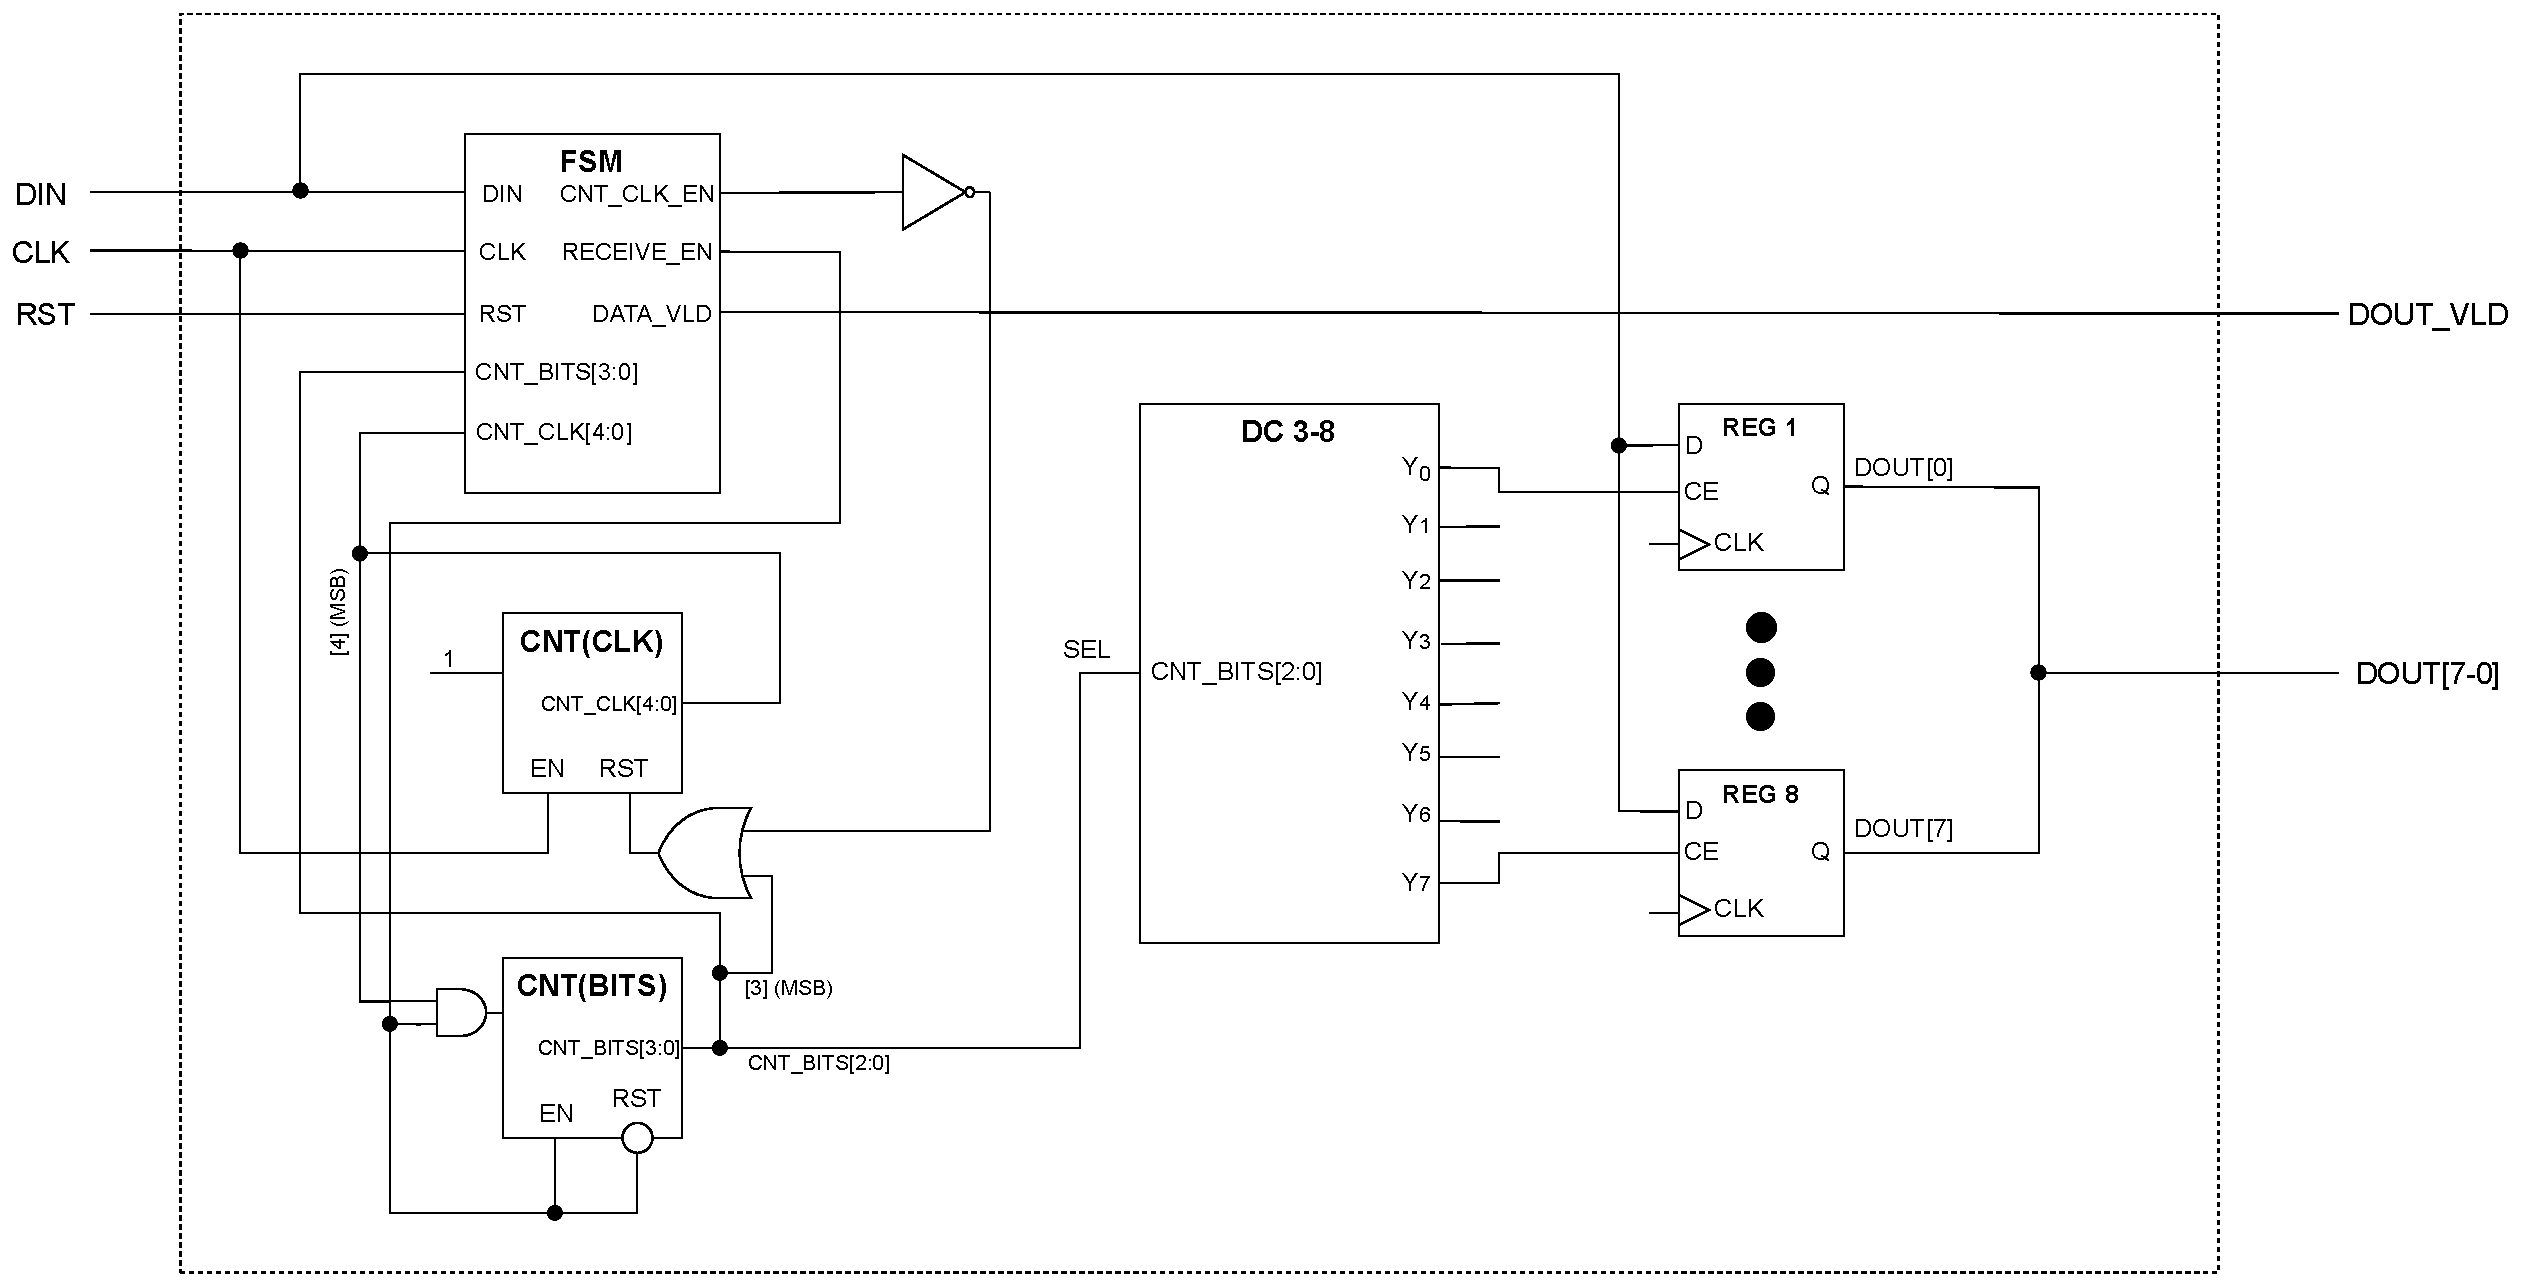
\includegraphics{schema.pdf}}
\end{centering}
\subsection{Popis}

Počítadlo\texttt{ CNT(CLK) }počítá hodinové signály následovně: je ve stavu\texttt{ RST}, když není nastaven\texttt{ CNT\_CLK\_EN }anebo když máme poslední načtený bit.
    
Počítadlo\texttt{ CNT(BITS) }počítá bity následovně: na vstupu má 1, pokud zároveň máme nastaveno\texttt{ RECEIVE\_EN }a když minulo 16 hodinových signálů.

Dál pomocí decóderu\texttt{ DC 3\,-\,8 } uchováváme do registrů\texttt{ REG 1\,-\,REG 8 }bity ze vstupu.

\newpage
\section{Návrh automatu (Finite State Machine)}
\subsection{Schéma automatu}
\begin{centering}
\scalebox{0.57}{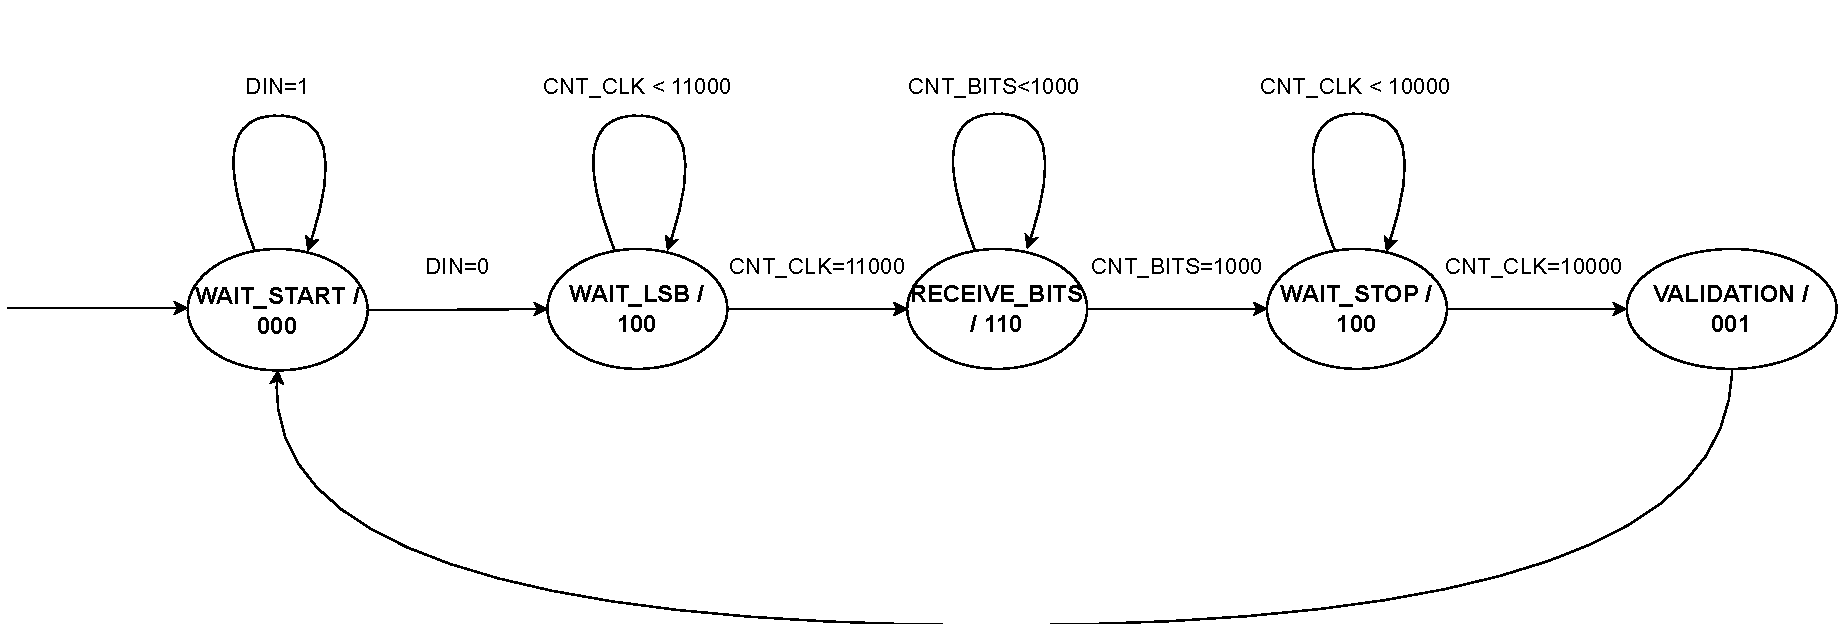
\includegraphics{fsm.pdf}}
\end{centering}
\subsection{Legenda}
\begin{itemize}
    \item Stavy automatu:\texttt{ WAIT\_START},\texttt{ WAIT\_LSB},\texttt{ RECEIVE\_BITS},\texttt{ WAIT\_STOP},\texttt{ VALIDATION}.
    
    \item Vstupní signály:\texttt{ DIN},\texttt{ CNT\_CLK},\texttt{ CNT\_BITS}.
    
    \item Moorovy výstupy (v tomto pořádí jsou vypsané v FSM):\texttt{ CNT\_CLK\_EN},\texttt{ RECEIVE\_EN},\texttt{ DATA\_VLD}.
\end{itemize}
\subsection{Popis}
\begin{itemize}
    \item \texttt{WAIT\_START}: čekáme na nastavení START bitu na 0.
    \item \texttt{WAIT\_LSB}: začátek přenosu\,--\,počítáme 1,5 period (celkem 24 signálů)\texttt{ CLK}, abychom dosáhli \uv{středu} LSB.
    \item \texttt{RECEIVE\_BITS}: uchováváme do registrů vstupní bity, dokud neni je 8.
    \item \texttt{WAIT\_STOP}: data jsou uložena, čekáme na nastavení STOP bitu na 1.
    \item \texttt{VALIDATION}: provádí se validace\,--\,nastavení\texttt{ DOUT\_VLD }na 1. Konec cyklu, přechod do stavu\texttt{ WAIT\_START}.
\end{itemize}

\newpage
\section{Snímek obrazovky ze simulací}
\begin{centering}
\hfill
\scalebox{0.9}{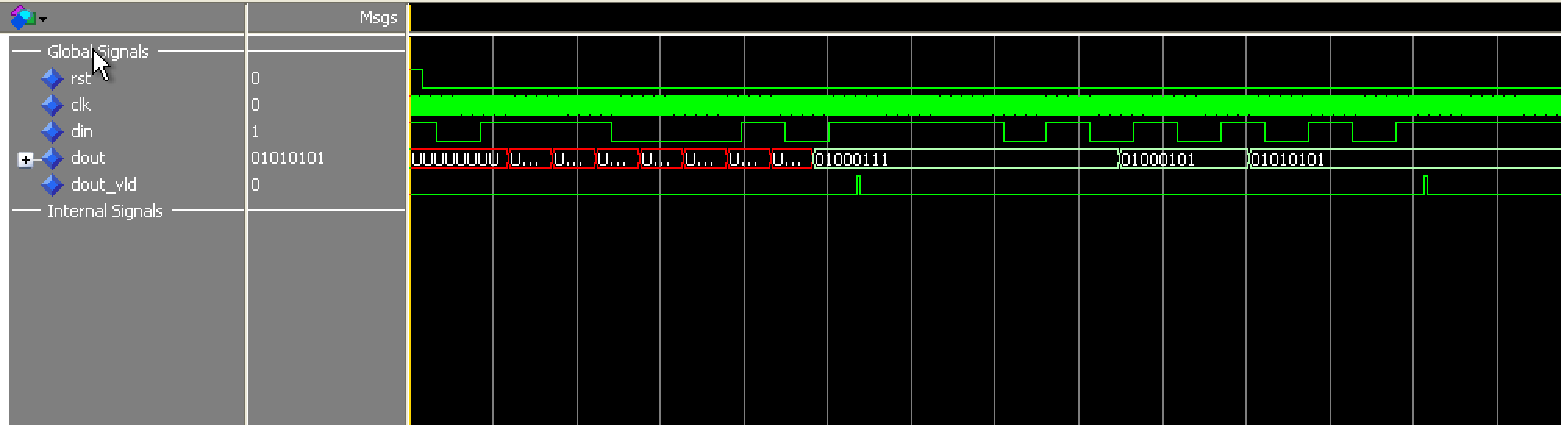
\includegraphics[angle=90]{obrazovka.pdf}}
\hfill
\end{centering}
\end{document}
